\documentclass{beamer}
%\usepackage{xspace}
\usepackage{amsmath,amssymb}
\usepackage{graphicx}
%\usepackage{svg}
%\usepackage{pgfpages}
%\pgfpagesuselayout{4 on 1}[a4paper,border shrink=5mm,landscape]
%\usepackage{psfrag}
%\usepackage[usenames,dvipsnames]{xcolor}
\usepackage{braket}
\usepackage{tikz}
\usepackage{tikz-3dplot}
%\usetikzlibrary{tikz-3dplot}
\usetikzlibrary{graphs}
\usetikzlibrary{datavisualization}
\usetikzlibrary{datavisualization.formats.functions}
\usepackage{pgfplotstable}
\usepgfplotslibrary{patchplots}

\setbeamercovered{transparent}

\usetheme{Pittsburgh}
%\usetheme{default}

\setbeamertemplate{sidebar right}{}
\setbeamertemplate{footline}[frame number]
%\usefonttheme{professionalfonts}

%\usepackage{sansmathaccent}
%\usepackage{bm}

%\usepackage{unicode-math}
%%\setmainfont[SlantedFont={Latin Modern Roman Slanted},SlantedFeatures={Color=000000},
%%  SmallCapsFont={TeX Gyre Termes},SmallCapsFeatures={Letters=SmallCaps}]{XITS}
%\setmathfont[math-style=ISO,sans-style=upright]{XITS Math}
%\setmathfont[range={\mathcal,\mathbfcal}]{Latin Modern Math}

%\usepackage{sfmath}

%\mathversion{sans}

\newcommand{\Tr}{\mathsf{Tr}}

\definecolor{redorange}{rgb}{1.0, .25, .25}
\definecolor{citation}{rgb}{.1, 0.8, .35}
\newcommand\emm[1]{\textcolor{redorange}{{#1}}}
\newcommand\numc[1]{\textcolor{citation}{{\bf #1}}}

%\newcommand\bm[1]{{\mbox{\boldmath $#1$}}}
\newcommand\bm[1]{{\mathbf{#1}}}
%\newcommand\bm[1]{{\bf #1}}
%\newcommand\bm[1]{\ensuremath{\boldsymbol{#1}}}
%\newcommand\bm[1]{{\textbf{\it #1}}}

\title{A single qubit}
\author{Ryuhei Mori}
%\institute{$\vcenter{\hbox{\includegraphics[width=30pt]{ELC_logo}}}$ Postdoctoral Fellow of ELC\\ $\vcenter{\hbox{\includegraphics[width=20pt]{titech_logo}}}$ Tokyo Institute of Technology}
\institute{Tokyo Institute of Technology}
\date{}



\begin{document}
\begin{frame}[plain]
\maketitle
\end{frame}

%\begin{frame}{Operation in a system}
%We will manipulate quantum state.
%
%\vspace{2em}
%This operation can be represented by a map $T: \text{Set of states} \to \text{Set of states}$.
%
%\vspace{2em}
%\end{frame}

\begin{frame}{A single bit}
Let $u:=\begin{bmatrix}1\\1\end{bmatrix}$.
\begin{itemize}
\setlength{\itemsep}{2em}
%\item State: \texttt{0},  \texttt{1} and their probabilistic mixture.
%\item Binary measurement: \texttt{0?}, \texttt{1?} and ther linear combination with coefficients in $[0,1]$.
\item 
%\begin{equation*}
$\text{Set of states} = \left\{\omega\in\mathbb{R}^2 \mid \omega\in C_{\ge 0}, \langle u, \omega\rangle = 1\right\}$.
%\end{equation*}
\item 
%\begin{equation*}
$\text{Set of binary measurements} = \left\{e\in\mathbb{R}^2 \mid e\in C_{\ge 0}, u-e \in C_{\ge 0} \right\}$.
%\end{equation*}
\end{itemize}

\vspace{3em}
\centering
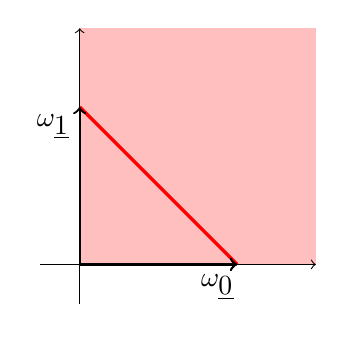
\begin{tikzpicture}
\draw[pink, fill] (0,0) rectangle +(3,3);
\draw[->] (-0.5,0) -- (3,0);
\draw[->] (0,-0.5) -- (0,3);
\draw[very thick, red] (2,0) -- (0,2);
\draw[->, thick] (0,0) -- node[anchor=north, very near end] {$\omega_{\underbar{0}}$} (2,0);
\draw[->, thick] (0,0) -- node[anchor=east, very near end] {$\omega_{\underbar{1}}$} (0,2);
\draw[->, thick] (0,0) -- (2,0);
\end{tikzpicture}
\hfill
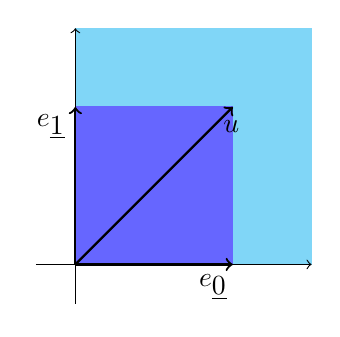
\begin{tikzpicture}
\draw[cyan!50, fill] (0,0) rectangle +(3,3);
\draw[blue!60, fill] (0,0) rectangle +(2,2);
\draw[->] (-0.5,0) -- (3,0);
\draw[->] (0,-0.5) -- (0,3);
%\draw (0,0) -- (2,2);
\draw[->, thick] (0,0) -- node[anchor=north, very near end] {$e_{\underbar{0}}$} (2,0);
\draw[->, thick] (0,0) -- node[anchor=east, very near end] {$e_{\underbar{1}}$} (0,2);
\draw[->, thick] (0,0) -- node[anchor=west, very near end] {$u$} (2,2);
\end{tikzpicture}

%Operation
%\begin{itemize}
%\item Identity: \texttt{0} $\mapsto$ \texttt{0}, \texttt{1} $\mapsto$ \texttt{1}
%\item Bit flip: \texttt{0} $\mapsto$ \texttt{1}, \texttt{1} $\mapsto$ \texttt{0}
%\end{itemize}
\end{frame}

\def\ysample{50}
\def\xsample{20}

\begin{frame}{A single qubit}
Let $u:=\begin{bmatrix}1&0\\0&1\end{bmatrix}$ and $\langle e,\omega\rangle := \Tr(e\omega)$.
\begin{itemize}
\setlength{\itemsep}{2em}
%\item State: A $2\times 2$ Hermitian matrix $\rho$ satisfying $\rho\succeq0$ and $\Tr(\rho)=1$.
%\item Binary measurements: A $2\times 2$ Hermitian matrix $\rho$ satisfying $\rho\succeq0$ and $I-\rho\succeq0$.
\item $\text{Set of states} = \left\{\omega\in V \mid \omega\in C_{\succeq 0}, \langle u,\omega\rangle = 1\right\}$.
\item $\text{Set of binary measurements} = \left\{e\in V \mid e\in C_{\succeq 0}, u-e \in C_{\succeq 0} \right\}$.
\end{itemize}
\begin{tikzpicture}
    \begin{axis}[height= 0.55\vsize, axis lines=center, axis on top, xmin=-1.0, xmax=1.0, ymin=-1.0, ymax=1.0, z buffer = sort, xtick = \empty, ytick=\empty, ztick=\empty ]
    \addplot3[surf, samples= \xsample, samples y=\ysample, domain= 0:1/sqrt(2), domain y= 0:2*pi, colormap = {pinkpink}{color=(pink) color=(pink)}]
      ({x*cos(deg(y))}, {x*sin(deg(y))}, {x});
    \addplot3[surf, samples= \xsample, samples y=\ysample, domain= 0:1/sqrt(2), domain y= 0:2*pi, color = red ]
      ({x*cos(deg(y))}, {x*sin(deg(y))}, {1/sqrt(2)});
    \end{axis}
\end{tikzpicture}
\begin{tikzpicture}
    \begin{axis}[height=0.70\vsize, axis lines=center, axis on top, xmin=-1.0, xmax=1.0, ymin=-1.0, ymax=1.0, z buffer = sort, xtick = \empty, ytick=\empty, ztick=\empty ]
    \addplot3[surf, samples= 2*\xsample, samples y=\ysample, domain= 0:sqrt(2), domain y= 0:2*pi, mesh/interior colormap = {blueblack}{color=(cyan!50) color=(cyan!50)}, colormap = {blueblack}{color=(blue!60) color=(blue!60)}]
      ({(sqrt(2)/2-abs(sqrt(2)/2-x))*cos(deg(y))}, {(sqrt(2)/2-abs(sqrt(2)/2-x))*sin(deg(y))}, {x});
    \end{axis}
\end{tikzpicture}
\end{frame}

\begin{frame}{A single qubit}
\begin{itemize}
\setlength{\itemsep}{3em}
\item A qubit can be represented by
\begin{equation*}
\rho = \frac12\left(I + r_X X + r_Y Y + r_Z Z\right)
\end{equation*}
for $[r_X\  r_Y\  r_Z]\in\mathbb{R}^3$ satisfying $r_X^2+r_Y^2+r_Z^2\le 1$.
\item A qubit can be represented by a point $[r_X\ r_Y\ r_Z]$ in a three-dimensional sphere of radius 1.
\end{itemize}
\end{frame}

\begin{frame}{The Bloch sphere}
\centering

\tdplotsetmaincoords{70}{120}
\begin{tikzpicture}[tdplot_main_coords, scale=2]

%\shade[ball color = lightgray, opacity = 0.5] (0,0,0) circle (1cm);

\tdplotsetrotatedcoords{20}{80}{0}
\draw[very thick, tdplot_rotated_coords] (0,0,0) circle (1);
%\begin{scope}[canvas is zx plane at y=0]
\draw[dashed, thick] (0,0,0) circle (1);
%\end{scope}
 
\draw[-stealth] (0,0,0) -- (2.00,0,0) node[below left] {$X$};
\draw[-stealth] (0,0,0) -- (0,1.80,0) node[below right] {$Y$};
\draw[-stealth] (0,0,0) -- (0,0,1.50) node[above] {$Z$};
 
\end{tikzpicture}
\end{frame}

\begin{frame}{Complex space and Hermitian operator}
\begin{itemize}
\item $\mathcal{X}$: A finite-dimensional inner product space on $\mathbb{C}$.
\item $\mathcal{L}(\mathcal{X})$: A set of linear operators on $\mathcal{X}$.
\end{itemize}

\vspace{1em}
For $A\in\mathcal{L}(\mathcal{X})$, an \emm{adjoint} map $A^\dagger$ of $A$ is a unique operator satisfying
\begin{equation*}
\langle v, Aw\rangle = \langle A^\dagger v, w\rangle
\end{equation*}
for any $v,\,w\in\mathcal{X}$.
$H\in\mathcal{L}(\mathcal{X})$ is Hermitian if and only if $H^\dagger = H$.
%$H\in\mathcal{L}(\mathcal{X})$ is Hermitian if and only if
%\begin{equation*}
%\langle v, Hw\rangle = \langle Hv, w\rangle
%\end{equation*}
%for any $v,\,w\in\mathcal{X}$.

\vspace{1em}
\begin{itemize}
\item $\mathcal{H}(\mathcal{X})$: A set of Hermitian operators on $\mathcal{X}$.
\end{itemize}

\vspace{2em}
$\mathcal{L}(\mathcal{X})$ and $\mathcal{H}(\mathcal{X})$ are often regarded as inner product space on $\mathbb{C}$ and $\mathbb{R}$, respectively
for the Hilbert--Schmidt inner product $\langle A, B\rangle = \Tr(A^\dagger B)$.
\end{frame}

\begin{frame}{Spectral decomposition theorem}
\begin{definition}[Normal operator]
$A\in\mathcal{L}(\mathcal{X})$ is said to be \emm{normal} if $AA^\dagger = A^\dagger A$.
\end{definition}

\vspace{1em}
Hermitian matrix ($H^\dagger = H$) and unitary matrix ($UU^\dagger = I$) are normal.

\vspace{2em}
\begin{theorem}[Spectral decomposition theorem]
$A\in \mathcal{L}(\mathbb{C}^n)$ is \emm{normal} if and only if there exist orthonormal basis $\{\ket{\psi_j}\}$ of $\mathbb{C}^n$ and complex numbers $\{\lambda_j\}$ such that
\begin{equation*}
A=\sum_j \lambda_j\ket{\psi_j}\bra{\psi_j}.
\end{equation*}
\end{theorem}
\end{frame}


\if0
\begin{frame}{Orthogonal projection}
Let $\mathcal{X}$ be a linear space. Let $\mathcal{Y}$ be a linear subspace of $\mathcal{X}$.
An orthogonal projection $\Pi_\mathcal{Y}\in\mathcal{H}(\mathcal{X})$ is defined by
\begin{itemize}
\item $\Pi_\mathcal{Y} v \in\mathcal{Y}$ for any $v\in\mathcal{X}$.
\item $\Pi_\mathcal{Y} v  = v$ for any $v\in\mathcal{Y}$.
\item $\Pi_\mathcal{Y}^2 = \Pi_\mathcal{Y}$.
\end{itemize}
\end{frame}

\begin{frame}{Spectral decomposition of Hermitian matrices}
$\mathsf{Ker}(H) \perp \mathsf{Im}(H)$.
For any $w\in\mathsf{Ker}(H)$ and $v\in\mathcal{X}$.
\begin{align*}
\langle Hv, w\rangle = \langle v, Hw\rangle = 0.
\end{align*}
Then, $H=(\Pi_{\mathsf{Ker}(H)}+\Pi_{\mathsf{Im}(H)})H(\Pi_{\mathsf{Ker}(H)}+\Pi_{\mathsf{Im}(H)})$.
For arbitrary $v\in\mathcal{X}$, $v,\,Hv,\,H^2v,\,\cdots H^nv$ are linearly dependent, i.e., there exists $a_0,\dotsc,a_n$ such that
\begin{equation*}
a_0v + a_1Hv + a_2H^2 v+ \dotsb + a_n H^n v = 0
\end{equation*}
\end{frame}
\fi

\begin{frame}{Pauli matrices}
\begin{itemize}
\setlength{\itemsep}{3em}
\item 
\begin{equation*}
Z=\begin{bmatrix}1&0\\0&-1\end{bmatrix}=
\begin{bmatrix}1\\0\end{bmatrix}\begin{bmatrix}1&0\end{bmatrix}
-\begin{bmatrix}0\\1\end{bmatrix}\begin{bmatrix}0&1\end{bmatrix}
\end{equation*}
\item 
\begin{equation*}
X=\begin{bmatrix}0&1\\1&0\end{bmatrix}=
\frac12\begin{bmatrix}1\\1\end{bmatrix}\begin{bmatrix}1&1\end{bmatrix}
-\frac12\begin{bmatrix}1\\-1\end{bmatrix}\begin{bmatrix}1&-1\end{bmatrix}
\end{equation*}
\item 
\begin{equation*}
Y=\begin{bmatrix}0&-i\\i&0\end{bmatrix}=
\frac12\begin{bmatrix}1\\i\end{bmatrix}\begin{bmatrix}1&-i\end{bmatrix}
-\frac12\begin{bmatrix}1\\-i\end{bmatrix}\begin{bmatrix}1&i\end{bmatrix}
\end{equation*}
\end{itemize}
\end{frame}

\begin{frame}{Braket notation}
\begin{align*}
\ket{0} &:= \begin{bmatrix}1\\0\end{bmatrix},&
\ket{1} &:= \begin{bmatrix}0\\1\end{bmatrix}
\end{align*}
\begin{align*}
\ket{+} &:= \frac1{\sqrt{2}}\begin{bmatrix}1\\1\end{bmatrix},&
\ket{-} &:= \frac1{\sqrt{2}}\begin{bmatrix}1\\-1\end{bmatrix}\\
&=\frac1{\sqrt{2}}(\ket{0}+\ket{1}),&
&=\frac1{\sqrt{2}}(\ket{0}-\ket{1})
\end{align*}
\begin{align*}
\ket{\psi} = \alpha\ket{0}+\beta\ket{1}=\begin{bmatrix}\alpha\\\beta\end{bmatrix}
\end{align*}
for $|\alpha|^2+|\beta|^2=1$.
\begin{align*}
\bra{\psi} = \ket{\psi}^\dagger = \alpha^*\bra{0}+\beta^*\bra{1}=\begin{bmatrix}\alpha^*&\beta^*\end{bmatrix}
\end{align*}
\end{frame}

\begin{frame}{Pauli matrices in braket notation}
\begin{itemize}
\setlength{\itemsep}{3em}
\item 
\begin{equation*}
Z=\begin{bmatrix}1&0\\0&-1\end{bmatrix}=
\ket{0}\bra{0}
-\ket{1}\bra{1}
\end{equation*}
\item 
\begin{equation*}
X=\begin{bmatrix}0&1\\1&0\end{bmatrix}=
\ket{+}\bra{+}
-\ket{-}\bra{-}
\end{equation*}
\item 
\begin{equation*}
Y=\begin{bmatrix}0&-i\\i&0\end{bmatrix}=
\frac12\begin{bmatrix}1\\i\end{bmatrix}\begin{bmatrix}1&-i\end{bmatrix}
-\frac12\begin{bmatrix}1\\-i\end{bmatrix}\begin{bmatrix}1&i\end{bmatrix}
\end{equation*}
\end{itemize}
\end{frame}

\begin{frame}{Special states}
\begin{equation*}
\rho = \frac12\left(I + r_X X + r_Y Y + r_Z Z\right)
\end{equation*}
\centering
$r_X^2+r_Y^2+r_Z^2\le 1$.

\vspace{1em}
\renewcommand{\arraystretch}{1.5}
\begin{tabular}{|c|c|}
\hline
Coordinate & State\\
\hline
$[0\ 0\ 0]$ & $\frac12 I$\\
$[1\ 0\ 0]$ & $\frac12 (I+X)=\ket{+}\bra{+}$\\
$[-1\ 0\ 0]$ & $\frac12 (I-X)=\ket{-}\bra{-}$\\
$[0\ 0\ 1]$ & $\frac12 (I+Z)=\ket{0}\bra{0}$\\
$[0\ 0\ -1]$ & $\frac12 (I-Z)=\ket{1}\bra{1}$\\
\hline
\end{tabular}
\end{frame}

\begin{frame}{Special states in the Bloch sphere}
\centering

\tdplotsetmaincoords{70}{120}
\begin{tikzpicture}[tdplot_main_coords, scale=2]

%\shade[ball color = lightgray, opacity = 0.5] (0,0,0) circle (1cm);

\tdplotsetrotatedcoords{20}{80}{0}
\draw[very thick, tdplot_rotated_coords] (0,0,0) circle (1);
%\begin{scope}[canvas is zx plane at y=0]
\draw[dashed, thick] (0,0,0) circle (1);
%\end{scope}
 
\draw[-stealth] (0,0,0) -- (2.00,0,0) node[below left] {$X$};
\draw[-stealth] (0,0,0) -- (0,1.80,0) node[below right] {$Y$};
\draw[-stealth] (0,0,0) -- (0,0,1.50) node[above] {$Z$};

\filldraw (0,0,0) circle (1pt) node[right] {$I/2$};
\filldraw (1,0,0) circle (1pt) node[below] {$\ket{+}\bra{+}$};
\filldraw (-1,0,0) circle (1pt) node[above] {$\ket{-}\bra{-}$};
\filldraw (0,0,1) circle (1pt) node[above] {$\ket{0}\bra{0}$};
\filldraw (0,0,-1) circle (1pt) node[below] {$\ket{1}\bra{1}$};
 
\end{tikzpicture}
\end{frame}

\if0
\begin{frame}{Spectral decomposition}
\end{frame}
\fi

\begin{frame}{Pure states are rank-1 density operators}
%\begin{definition}
\vspace{-.5em}
\begin{align*}
& \text{$\rho$ is a \emm{pure state}}\\
& \overset{\text{def}}{\iff} \rho\ne p\rho_1+(1-p)\rho_2\quad \forall p\in(0,1) \text{ and states $\rho_1 \ne \rho_2$}.
\end{align*}
\begin{lemma}
A quantum state $\rho$ is a pure state if and only if $\rho$ is \emm{rank-1}.
\end{lemma}
\begin{proof}
\small
Let the spectral decomposition of $\rho$ be
\begin{equation*}
\rho=\sum_j \lambda_j\ket{\psi_j}\bra{\psi_j}
\end{equation*}
where $\lambda_j\ge 0$ and $\sum_j\lambda_j = 1$.
If $\rho$ is not rank-1, $\rho$ is a convex combination of quantum states $(\ket{\psi_j}\bra{\psi_j})_j$.

Assume $\rho=\ket{\varphi}\bra{\varphi}$ and $\rho=p_1\rho_1+p_2\rho_2$.
$\Tr(\sigma\ket{\varphi}\bra{\varphi})=1$ if and only if $\sigma=\ket{\varphi}\bra{\varphi}$ since $\Tr(\sigma \ket{\varphi}\bra{\varphi})=\bra{\varphi}\sigma\ket{\varphi} = \sum_j \lambda_j |\braket{\psi_j|\varphi}|^2$.
%Assume that $\rho=\ket{\varphi}\bra{\varphi}$ and $\rho = p\rho_1+(1-p)\rho_2$.
Then, $\Tr((p_1\rho_1+p_2\rho_2)\ket{\varphi}\bra{\varphi})=1$ implies that $\Tr(\rho_1\ket{\varphi}\bra{\varphi})=\Tr(\rho_2\ket{\varphi}\bra{\varphi})=1$, and hence $\rho_1=\rho_2=\rho$.
\end{proof}
%\end{definition}
\end{frame}

\begin{frame}{Pure states and state vector}
Pure state $\ket{\psi}\bra{\psi}$ can be represented by a \emm{state vector} $\ket{\psi}\in\mathbb{C}^2$ with $\braket{\psi|\psi}=1$.

\vspace{.7em}
$\ket{\psi}$ and $\ket{\varphi}:=\mathsf{e}^{i\theta}\ket{\psi}$ represent the same state since $\ket{\psi}\bra{\psi}=\ket{\varphi}\bra{\varphi}$.
\end{frame}

\begin{frame}{Inner product of pure states}
\begin{itemize}
\item $\rho$ is a qubit pure state with a coordinate $[r_X\ r_Y\ r_Z]$.
\item $\sigma$ is a qubit pure state with a coordinate $[-r_X\ -r_Y\ -r_Z]$.
\end{itemize}
\begin{align*}
\Tr(\rho\sigma) =
\Tr(\rho(I-\rho)) =
\Tr(\rho)-\Tr(\rho^2) =1-1=0
\end{align*}

\vspace{2em}
\begin{itemize}
\item $\rho=\ket{\psi}\bra{\psi}$.
\item $\sigma=\ket{\varphi}\bra{\varphi}$.
\end{itemize}
\begin{align*}
\Tr(\rho\sigma) &=
\Tr(\ket{\psi}\bra{\psi}\ket{\varphi}\bra{\varphi}) =
\braket{\psi|\varphi}\Tr(\ket{\psi}\bra{\varphi})\\
 &= \braket{\psi|\varphi}\braket{\varphi|\psi}
 = |\braket{\psi|\varphi}|^2
\end{align*}
\end{frame}

\begin{frame}{Single qubit measurement}
\begin{align*}
\text{Set of measurements} = \{(e_1,\dotsc,e_k) &\mid e_1+\dotsb+e_k=I, e_j\in C_{\succeq 0}\\
&i=1,2,\dotsc,k,\, k=1,2,\dotsc\}
\end{align*}
If $e_i e_j = \delta_{i,j}e_i$, the measurement is called an \emm{orthogonal measurement}.

\vspace{1em}
If $\ket{0}\bra{0}$ is measured by $(\ket{0}\bra{0}, \ket{1}\bra{1})$,
the output is 0 with probability $\Tr(\ket{0}\bra{0} \ket{0}\bra{0})=|\braket{0|0}|^2=1$.

\vspace{1em}
If $\ket{+}\bra{+}$ is measured by $(\ket{0}\bra{0}, \ket{1}\bra{1})$,
the output is 0 with probability $\Tr(\ket{0}\bra{0} \ket{+}\bra{+})=|\braket{0|+}|^2=1/2$.

\vspace{1em}
If $\ket{\psi}\bra{\psi}$ is measured by $(\ket{\varphi_0}\bra{\varphi_0}, \ket{\varphi_1}\bra{\varphi_1})$,
the output is 0 with probability $\Tr(\ket{\varphi_0}\bra{\varphi_0} \ket{\psi}\bra{\psi})=|\braket{\varphi_0|\psi}|^2$.
\end{frame}

\begin{frame}{Quantum channel}
\end{frame}

\begin{frame}{Single qubit quantum channel}
Since real vector space spanned by 2x2 Hermitian matrices is 4-dimensional, any linear map $\Phi$ on the linear space
is represented by 4x4 real matrix.
\begin{align*}
\Phi\left(\bm{a}\cdot \bm{\sigma}\right)
=
(T\bm{a})\cdot \bm{\sigma}
\end{align*}
Here,
\begin{align*}
T_{i,j} = \frac12\Tr(\sigma_i\Phi(\sigma_j)).
\end{align*}
From the trace-preserving property
\begin{align*}
T_{0,0} &= \frac12\Tr(\Phi(I)) = \frac12\Tr(I) = 1,&
T_{0,1} &= \frac12\Tr(\Phi(X)) = \frac12\Tr(X) = 0.
\end{align*}
\begin{align*}
T &=
\begin{bmatrix}
1&0&0&0\\
t_1&\\
t_2&\\
t_3
\end{bmatrix}
\end{align*}
\end{frame}

\begin{frame}{Unitary operation}
For unitary operation $U$, let us consider
\begin{equation*}
\rho\mapsto U\rho U^\dagger.
\end{equation*}

\vspace{2em}
It is easy to see that
\begin{itemize}
\item $\Tr(U\rho U^\dagger)=1$
\item $U\rho U^\dagger\succeq 0$
\end{itemize}

\vspace{3em}
A pure state $\ket{\psi}$ is mapped to a pure state $U\ket{\psi}$.

\vspace{2em}
$U$ and $\mathsf{e}^{i\theta}U$ are physically equivalent.
\end{frame}

\begin{frame}{Matrix representation of unitary channel}
Unitary channel is \emm{unital}, i.e., $\Phi(I) = I$.

\begin{align*}
T_{1,0} &= \frac12\Tr(X\Phi(I)) = \frac12\Tr(X) = 0
\end{align*}

\begin{align*}
T &=
\begin{bmatrix}
1&0&0&0\\
0&\\
0&\\
0
\end{bmatrix}
\end{align*}

Unitary channel is represented by the 3x3 real matrix $M$.
\end{frame}

\begin{frame}{Examples of unitary operations}
\begin{itemize}
\setlength{\itemsep}{2em}
\item The identity matrix $I$.
\item Pauli matrices $X$, $Y$ and $Z$.
\item Hadamard matrix $H:=\frac1{\sqrt{2}}\begin{bmatrix}1&1\\1&-1\end{bmatrix}$
\item Product $UV$ of unitary operators $U$ and $V$.
\end{itemize}
\end{frame}

\begin{frame}{Multiplications of Pauli matrices}
For any unitary matrices $U$ and $V$, $UV$ is also unitary matrix.

\vspace{2em}
\begin{itemize}
\setlength{\itemsep}{2em}
\item $XY=iZ$
\item $YZ=iX$
\item $ZX=iY$
\end{itemize}
\end{frame}

\begin{frame}{Pauli matrices $X$ on the Bloch sphere}
\begin{equation*}
\rho = \frac12\left(I + r_X X + r_Y Y + r_Z Z\right)
\end{equation*}
\begin{align*}
X\rho X^\dagger &= X\rho X =  \frac12\left(X^2 + r_X X^3 + r_Y XYX + r_Z XZX\right)\\
&=  \frac12\left(I + r_X X - r_Y Y - r_Z Z\right)
\end{align*}
\begin{align*}
[r_X\ r_Y\ r_Z]\overset{X}{\longmapsto} [r_X\ -r_Y\ -r_Z]
\end{align*}
\emm{$\pi$-rotation} with respect to $X$ axis.
$M = \begin{bmatrix}1&0&0\\0&-1&0\\0&0&-1\end{bmatrix}$.

\vspace{1em}
Similarly, $Y$ and $Z$ corresponds to \emm{$\pi$-rotation} with respect to $Y$ and $Z$ axes, respectively.
\end{frame}

\begin{frame}{Hadamard matrix}
Hadamard matrix $H$ is unitary and Hermitian.
\begin{align*}
H:=\frac1{\sqrt{2}}\begin{bmatrix}1&1\\1&-1\end{bmatrix}
&=\ket{+}\bra{0}+\ket{-}\bra{1}\\
&=\ket{0}\bra{+}+\ket{1}\bra{-}
\end{align*}
\begin{align*}
\ket{0},\,\ket{1} \emm{\overset{H}{\longleftrightarrow}} \ket{+},\,\ket{-}
\end{align*}
\begin{align*}
HXH &= H(\ket{+}\bra{+}-\ket{-}\bra{-})H\\
&= \ket{0}\bra{0}-\ket{1}\bra{1} = Z
\end{align*}

Similarly, $HZH=X$.

$HYH=H(iXZ)H =i HXH HZH = i Z X= - Y$
\end{frame}

\begin{frame}{Hadamard matrix on the Bloch sphere}
\begin{equation*}
\rho = \frac12\left(I + r_X X + r_Y Y + r_Z Z\right)
\end{equation*}
\begin{align*}
H\rho H^\dagger &= H\rho H =  \frac12\left(H^2 + r_X HXH + r_Y HYH + r_Z HZH\right)\\
&=  \frac12\left(I + r_X Z - r_Y Y + r_Z X\right)
\end{align*}
\begin{align*}
[r_X\ r_Y\ r_Z]\overset{H}{\longmapsto} [r_Z\ -r_Y\ r_X]
\end{align*}
$M=\begin{bmatrix}0&0&1\\0&-1&0\\1&0&0\end{bmatrix}$.
%Hadamard operation can be decomposed to \emm{$\pi/2$-rotation} with respect to $Y$ axis
%\begin{align*}
%[r_X\ r_Y\ r_Z]\overset{R_Y(\pi/2)}{\longmapsto} [r_Z\ r_Y\ -r_X]
%\end{align*}
%and \emm{$X$}.
\end{frame}


\begin{frame}{Rotation matrices}
\small
\begin{equation*}
R_Z(\theta) := \cos\frac{\theta}2 I - i \sin\frac{\theta}2 Z
\end{equation*}
\begin{equation*}
R_X(\theta)^\dagger = R_X(-\theta)
\end{equation*}
\begin{align*}
R_X(\theta)R_X(\theta)^\dagger &= (\cos\frac{\theta}2 I - i \sin\frac{\theta}2 X)(\cos\frac{\theta}2 I + i \sin\frac{\theta}2 X)\\
&= \cos^2\frac{\theta}2 I + \sin^2\frac{\theta}2 X^2=I
\end{align*}
\begin{align*}
R_X(\theta)X&=X R_X(\theta),&
R_X(\theta)Y&=Y R_X(-\theta),&
R_X(\theta)Z&=Z R_X(-\theta)
\end{align*}
\begin{align*}
R_X(\theta)R_X(\tau)=R_X(\theta+\tau)
\end{align*}
\begin{align*}
[1\  0\  0]&\overset{R_X(\theta)}{\longmapsto} [1\ 0\ 0]\\
[0\  1\  0]&\overset{R_X(\theta)}{\longmapsto} [0\ \cos\theta\ \sin\theta]\\
[0\  0\  1]&\overset{R_X(\theta)}{\longmapsto} [0\ -\sin\theta\ \cos\theta]
\end{align*}
\emm{$\theta$-rotation} with respect to $X$ axis.
%\begin{align*}
%R_X(\theta)\rho R_X(\theta)^\dagger &= \frac12\left(I + r_X X + r_Y R_X(\theta)YR_X(\theta)^\dagger + r_Z R_X(\theta)ZR_X(\theta)^\dagger\right)\\
%&= ...
%\end{align*}
\end{frame}

\if0
\begin{frame}{Matrix function}
\begin{definition}
For $f\colon \mathbb{C}\to\mathbb{C}$ and orthonormal basis $(\ket{\psi_j})_j$ of $\mathcal{X}$,
\begin{equation*}
f\left(\sum_j \lambda_j \ket{\psi_j}\bra{\psi_j}\right) := \sum_j \emm{f(\lambda_j)} \ket{\psi_j}\bra{\psi_j}.
\end{equation*}
\end{definition}
For $H\in\mathcal{H}(\mathcal{X})$,
$\exp(iH)$ is unitary.

\vspace{2em}
Since the radius of convergense of $\exp$ at 0 is infinity,
\begin{equation*}
\exp(A) = \sum_{j=0}^\infty \frac1{j!}A^j.
\end{equation*}

\vspace{1em}
In general, $\exp(A+B)\ne\exp(A)\exp(B)$.
\end{frame}

\begin{frame}{General unitary matrix}
A normal matrix $U$ is unitary iff all eigenvalues of $U$ have absolute value 1
since for
\begin{equation*}
U=\sum_j \lambda_j\ket{\psi_j}\bra{\psi_j}.
\end{equation*}
it holds
\begin{equation*}
UU^\dagger=\sum_j |\lambda_j|^2\ket{\psi_j}\bra{\psi_j}.
\end{equation*}

Let $\lambda_j = \mathsf{e}^{i\theta_j}$.
Then, for Hermitian matrix
\begin{equation*}
H=\sum_j \theta_j\ket{\psi_j}\bra{\psi_j}.
\end{equation*}
$U = \emm{\exp(i H)}$.
\end{frame}
\fi

\begin{frame}{General unitary matrix}
$Tr(UAU^\dagger UBU^\dagger) = \Tr(AB)$.

$M$ is orthogonal matrix.

\vspace{2em}
Since for
\begin{equation*}
U=\sum_j \lambda_j\ket{\psi_j}\bra{\psi_j}= VR_Z(\theta)V^\dagger.
\end{equation*}
\begin{equation*}
M = S R S^{-1}
\end{equation*}
$\det(M)=1$
\end{frame}

\begin{frame}{Assignments}
\begin{enumerate}
\setlength{\itemsep}{2em}
\item For $a,b,c,d\in\mathbb{R}$, show $r_I,\ r_X,\ r_Y,\ r_Z\in\mathbb{R}$ satisfying $\begin{bmatrix}a&b+ci\\b-ci&d\end{bmatrix} = r_II+r_XX+r_YY+r_ZZ$.
\item Express $\exp\left(-i\frac{\theta}2 X\right)$ for $\theta\in\mathbb{R}$ as a complex linear combination of $I$, $X$, $Y$ and $Z$.
A summation with infinite number of terms is not allowed.
%\item Show that $R_Y(\theta):=\cos\frac{\theta}2-i\sin\frac{\theta}2Y=\begin{bmatrix}\cos\frac{\theta}2 & -\sin\frac{\theta}2\\ \sin\frac{\theta}2 & \cos\frac{\theta}2\end{bmatrix}$
%and $R_Z(\theta):=\cos\frac{\theta}2-i\sin\frac{\theta}2Z=\begin{bmatrix}\mathsf{e}^{-i\theta/2}&0\\0&\mathsf{e}^{i\theta/2}\end{bmatrix}$.
%\item Show that for any $2\times 2$ unitary matrix, there exist $\alpha,\,\beta,\,\gamma,\,\delta\in\mathbb{R}$ such that
%\begin{equation*}
%U=\mathsf{e}^{i\alpha}R_Z(\beta)R_Y(\gamma)R_Z(\delta)
%\end{equation*}
\item {[Advanced]} For $a_I,\ a_X,\ a_Y,\ a_Z\in\mathbb{R}$, represents
\begin{equation*}
\exp\left(i(a_II+a_XX+a_YY+a_ZZ)\right)
\end{equation*}
by a linear combination of $I, X, Y$ and $Z$.
A summation with infinite number of terms is not allowed.
\end{enumerate}
\end{frame}



\end{document}
